\documentclass{beamer}
\mode<presentation>
\usepackage{amsmath}
\usepackage{amssymb}
%\usepackage{advdate}
\usepackage{graphicx}
\usepackage{adjustbox}
\usepackage{subcaption}
\usepackage{enumitem}
\usepackage{multicol}
\usepackage{mathtools}
\usepackage{listings}
\usepackage{url}
\def\UrlBreaks{\do\/\do-}
\usetheme{Boadilla}
\usecolortheme{lily}
\setbeamertemplate{footline}
{
  \leavevmode%
  \hbox{%
  \begin{beamercolorbox}[wd=\paperwidth,ht=2.25ex,dp=1ex,right]{author in head/foot}%
    \insertframenumber{} / \inserttotalframenumber\hspace*{2ex} 
  \end{beamercolorbox}}%
  \vskip0pt%
}
\setbeamertemplate{navigation symbols}{}

\providecommand{\nCr}[2]{\,^{#1}C_{#2}} % nCr
\providecommand{\nPr}[2]{\,^{#1}P_{#2}} % nPr
\providecommand{\mbf}{\mathbf}
\providecommand{\pr}[1]{\ensuremath{\Pr\left(#1\right)}}
\providecommand{\qfunc}[1]{\ensuremath{Q\left(#1\right)}}
\providecommand{\sbrak}[1]{\ensuremath{{}\left[#1\right]}}
\providecommand{\lsbrak}[1]{\ensuremath{{}\left[#1\right.}}
\providecommand{\rsbrak}[1]{\ensuremath{{}\left.#1\right]}}
\providecommand{\brak}[1]{\ensuremath{\left(#1\right)}}
\providecommand{\lbrak}[1]{\ensuremath{\left(#1\right.}}
\providecommand{\rbrak}[1]{\ensuremath{\left.#1\right)}}
\providecommand{\cbrak}[1]{\ensuremath{\left\{#1\right\}}}
\providecommand{\lcbrak}[1]{\ensuremath{\left\{#1\right.}}
\providecommand{\rcbrak}[1]{\ensuremath{\left.#1\right\}}}
\theoremstyle{remark}
\newtheorem{rem}{Remark}
\newcommand{\sgn}{\mathop{\mathrm{sgn}}}
\providecommand{\abs}[1]{\vert#1\vert}
\providecommand{\res}[1]{\Res\displaylimits_{#1}} 
\providecommand{\norm}[1]{\lVert#1\rVert}
\providecommand{\mtx}[1]{\mathbf{#1}}
\providecommand{\mean}[1]{E[ #1 ]}
\providecommand{\fourier}{\overset{\mathcal{F}}{ \rightleftharpoons}}
%\providecommand{\hilbert}{\overset{\mathcal{H}}{ \rightleftharpoons}}
\providecommand{\system}[1]{\overset{\mathcal{#1}}{ \longleftrightarrow}}
%\providecommand{\system}{\overset{\mathcal{H}}{ \longleftrightarrow}}
	%\newcommand{\solution}[2]{\vec{Solution:}{#1}}
%\newcommand{\solution}{\noindent \vec{Solution: }}
\providecommand{\dec}[2]{\ensuremath{\overset{#1}{\underset{#2}{\gtrless}}}}
\newcommand{\myvec}[1]{\ensuremath{\begin{pmatrix}#1\end{pmatrix}}}


\lstset{
%language=C,
frame=single, 
breaklines=true,
columns=fullflexible
}
\lstset{
  language=C,
  basicstyle=\ttfamily\footnotesize,
  keywordstyle=\color{blue}\bfseries,
  commentstyle=\color{gray}\itshape,
  stringstyle=\color{orange},
  numbers=left,
  numberstyle=\tiny\color{gray},
  breaklines=true,
  frame=single,
  showstringspaces=false,
  tabsize=4,
  captionpos=b
}
\numberwithin{equation}{section}
\lstset{
  language=Python,
  basicstyle=\ttfamily\small,
  keywordstyle=\color{blue},
  stringstyle=\color{orange},
  numbers=left,
  numberstyle=\tiny\color{gray},
  breaklines=true,
  showstringspaces=false
}

\title{Problem 1.8.11}
\author{Sujal Rajani}

\date{\today} 
\begin{document}

\begin{frame}
\titlepage
\end{frame}

\section*{Outline}
\begin{frame}
\tableofcontents
\end{frame}
\section{Question}
\begin{frame}{Question}
\textbf{Question}:


\noindent AOBC is a rectangle whose three vertices are vertices $\vec{A}(0,3),\vec{O}(0,0),\vec{B}(5,0)$. The 
length of diagonal is \underline{\hspace{2cm}}.   

\end{frame}

    

\section{Solution}
\begin{frame}{Solution}
\textbf{Solution:} 
\\
From the given information,
\begin{align}
		\vec{A} = \myvec{0\\3},\vec{O} = \myvec{0\\0},\vec{B} = \myvec{5\\0} 
\end{align}
Then the direction vector  of the diagonal AB is :

\begin{align}
    \vec{A-B}=\myvec{0\\3}-\myvec{5\\0}=\myvec{-5\\3},
    \\
  \end{align}
the length of the diagonal is :
\begin{align}
    (\vec{A}-\vec{B})^T(\vec{A}-\vec{B})=34
    
    
    
    
    
     \Rightarrow AB=||\vec{A}-\vec{B}||=\sqrt{34}	 
    \end{align}
    \end{frame}
    \subsection{plot}
       \begin{frame}[fragile]
    \begin{figure}[H]
    \centering
    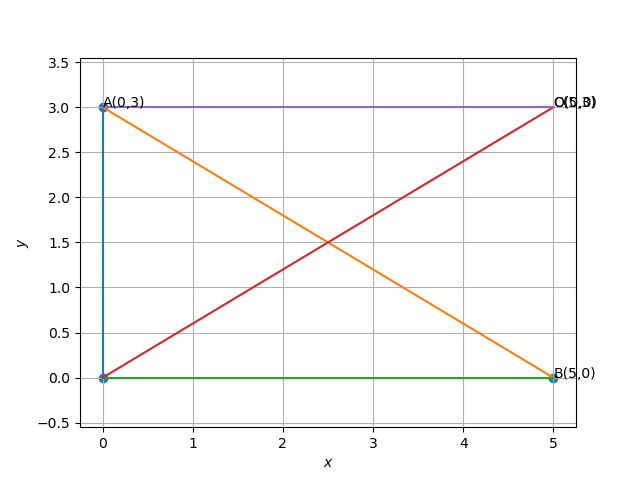
\includegraphics[width = 0.6\columnwidth]{../figs/img.png}
    \caption*{}
    \label{figs}
\end{figure}
\end{frame}
\section{ C Code}
\begin{frame}[fragile]
\frametitle{C Code }
\begin{lstlisting}[language=C]
#include <stdio.h>
#include <math.h>
#include <stdlib.h>
#include "libs/matfun.h"   // For createMat, freeMat

int main() {
    // Define points as column vectors
    double **A, **B;
    double dx, dy, diagonal;

    // Allocate 2x1 matrices for A and B
    A = createMat(2, 1);
    B = createMat(2, 1);

    // A = (0,3), B = (5,0)
    A[0][0] = 0;   A[1][0] = 3;
    B[0][0] = 5;   B[1][0] = 0;

    
\end{lstlisting}
\end{frame}

\begin{frame}[fragile]
\frametitle{C Code }
\begin{lstlisting}[language=C]

    // Calculate diagonal length = ||A - B||
    dx = A[0][0] - B[0][0];
    dy = A[1][0] - B[1][0];
    diagonal = sqrt(dx*dx + dy*dy);

    printf("Length of diagonal AB = %.2lf\n", diagonal);

    // Free matrices
    freeMat(A, 2);
    freeMat(B, 2);

    return 0;
}
\end{lstlisting}
\end{frame}

\begin{frame}[fragile]
\frametitle{Python Code for Plotting}
\begin{lstlisting}[language=Python]
    import math
import sys   

import numpy as np
import numpy.linalg as LA
import matplotlib.pyplot as plt
import matplotlib.image as mpimg
from line.funcs import *
#from triangle.funcs import *
#from conics.funcs import circ_gen
#if using termux
import subprocess
import shlex
#end if

A = np.array([0,3]).reshape(-1,1)
B = np.array([5,0]).reshape(-1,1)
O = np.array([0,0]).reshape(-1,1)
C = np.array([5,3]).reshape(-1,1)

\end{lstlisting}

\end{frame}
\section{Python Code}
\begin{frame}[fragile]
\frametitle{Python Code for Plotting}
\begin{lstlisting}[language=Python]   

coords = np.block([[A,B,O]])

AO = line_gen(A,O)
AB = line_gen(A,B)
BO = line_gen(B,O)
CO = line_gen(C,O)
AC = line_gen(A,C)
plt.plot(AO[0,:],AO[1,:])
plt.plot(AB[0,:],AB[1,:])
plt.plot(BO[0,:],BO[1,:])
plt.plot(CO[0,:],CO[1,:])
plt.plot(AC[0,:],AC[1,:])
plt.scatter(coords[0,:],coords[1,:])


plt.text(A[0],A[1],"A(0,3)")
plt.text(B[0],B[1],"B(5,0)")



\end{lstlisting}

\end{frame}
\begin{frame}[fragile]
\frametitle{Python Code for Plotting}
\begin{lstlisting}[language=Python]   

plt.text(C[0],C[1],"C(5,3)")
plt.text(C[0],C[1],"O(0,0)")
plt.xlabel('$x$')
plt.ylabel('$y$')
plt.legend(loc='best')
plt.grid() # minor
plt.axis('equal')

plt.savefig('../figs/img.png')


\end{lstlisting}

\end{frame}
\end{document}
